\subsection{Methodology}

The following sections report the performance of the code using differing numbers of MPI nodes. The \textit{nodes} in each chart refers to the command line parameter:

\texttt{mpirun -np} \textit{nodes} \texttt{./parallelSort}


\subsection{initializeMPI}

The \texttt{initializeMPI} section of code refers to performing the \texttt{MPI\_Init} call, \texttt{MPI\_Comm\_rank}, \texttt{MPI\_Comm\_size}, and \texttt{MPI\_Get\_processor\_name}. There is no reportable difference in performance based on the number of nodes requested.

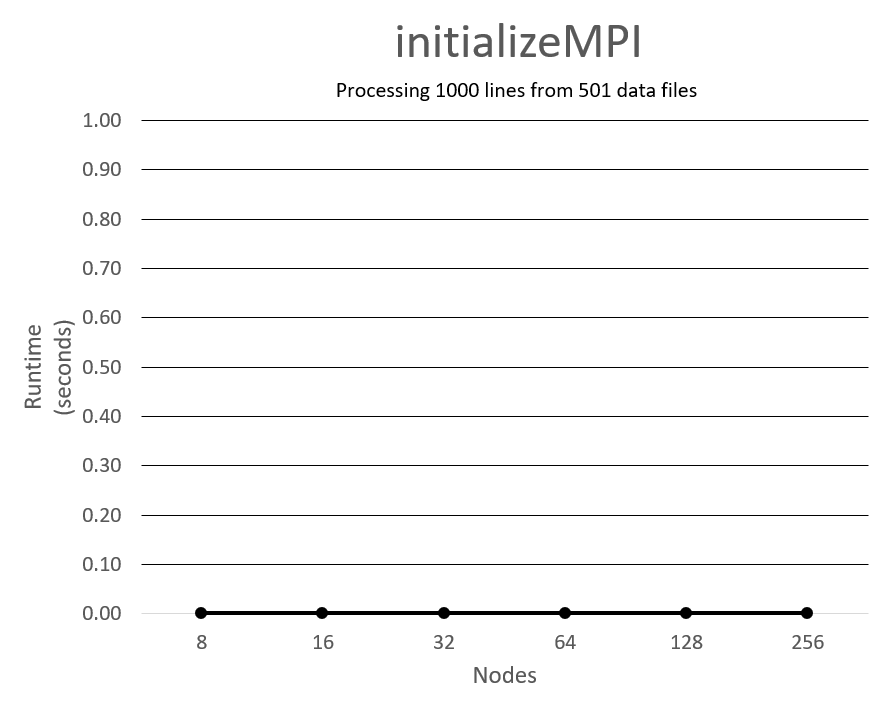
\includegraphics[width=0.8\textwidth]{initializeMPI.png}

\subsection{distributeFileNames}

This code reads the list of files in a directory matching the required pattern and distributes them to the worker nodes using \texttt{MPI\_Isend}. Timing ends when all nodes have completed their receives. As the number of nodes increases, the amount of time required grows exponentially. (\textit{Note: the x-axis is exponential by powers of two.})

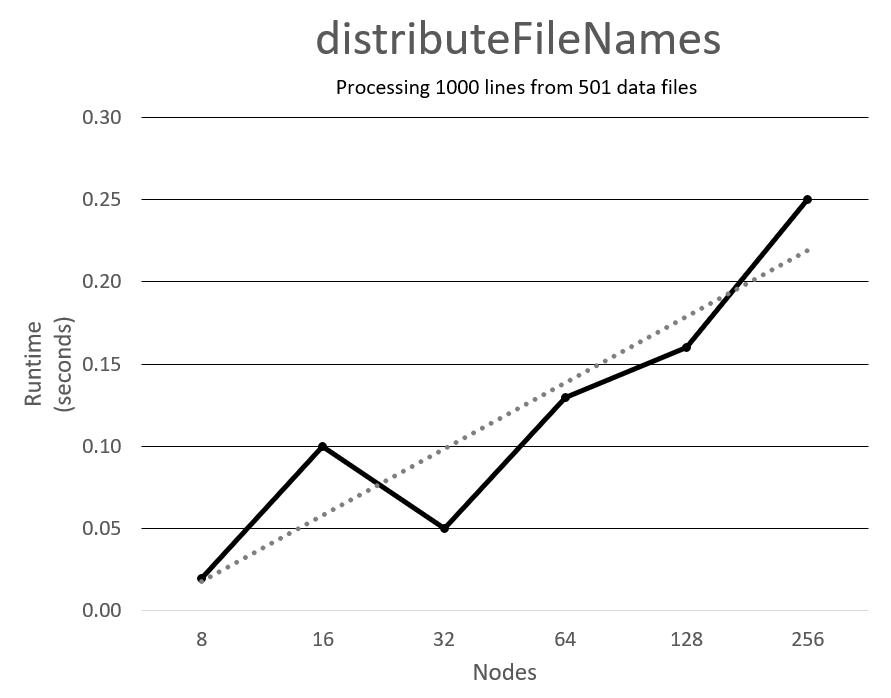
\includegraphics[width=0.8\textwidth]{distributeFileNames.png}

\subsection{importData}

This code performs a \texttt{while} loop reading each line from each file. The line is stored as a \texttt{string} and parsed using \texttt{substr} and \texttt{stod}.

The amount of time required to import files drops exponentially as the number of files any single node must process is reduced.

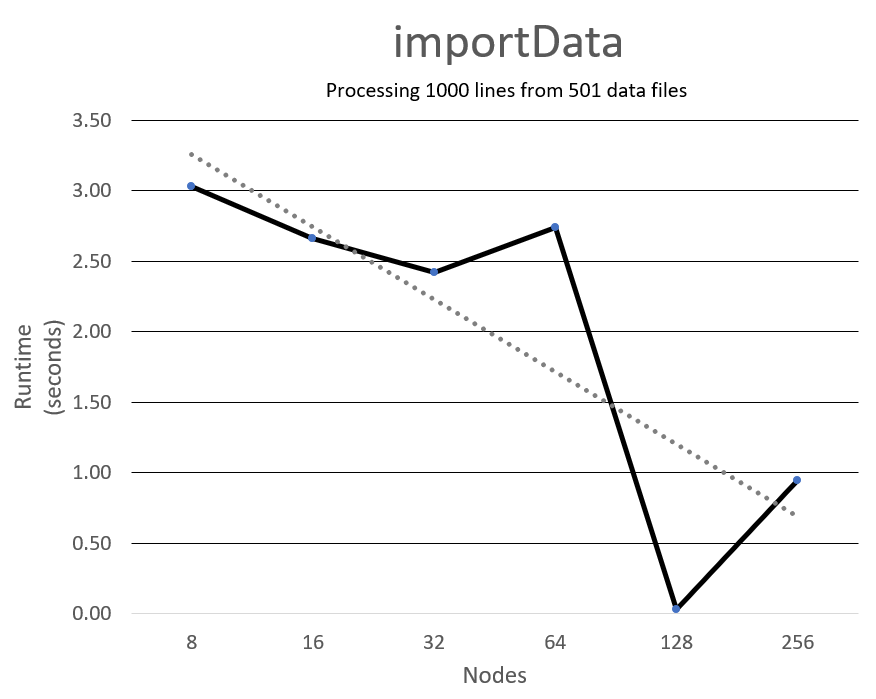
\includegraphics[width=0.8\textwidth]{importData.png}

\subsection{sortData}

The \texttt{sortData} function reorganizes the data in ascending order by the selected field. Like \texttt{importFiles}, the time to perform the sort falls exponentially since the amount of data is reduced.

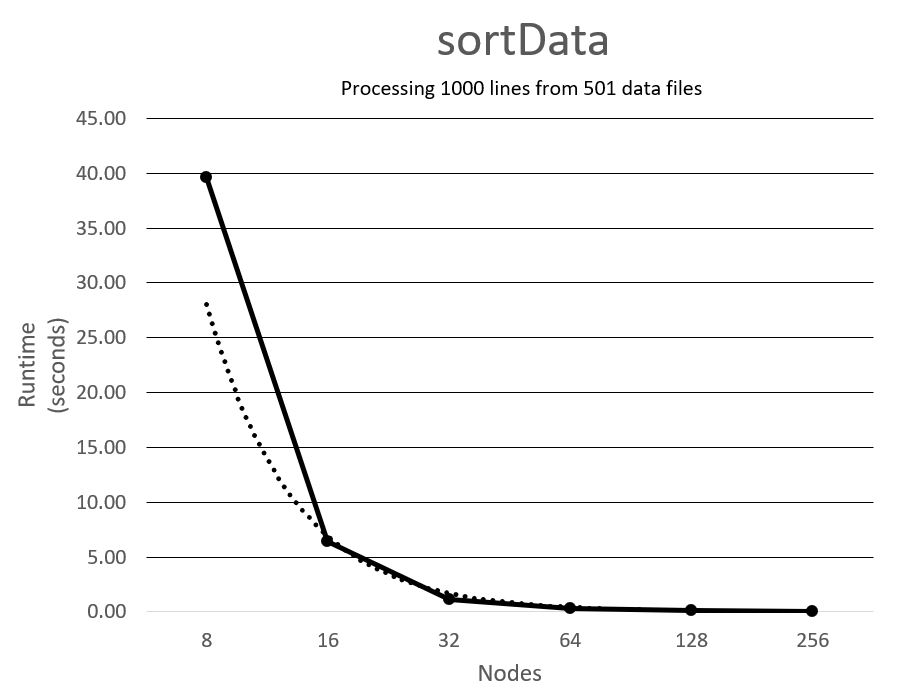
\includegraphics[width=0.8\textwidth]{sortData.png}

\subsection{adaptBins}

The \texttt{adaptBins} portion of the code appears to perform well until 256 nodes. Other sections of the code were experiencing significant performance issues at this scale, and it is possible that the problem may be related to the cluster's workload rather than the algorithm. Unfortunately, the old methods to validate this is to run the code without other users on the system.

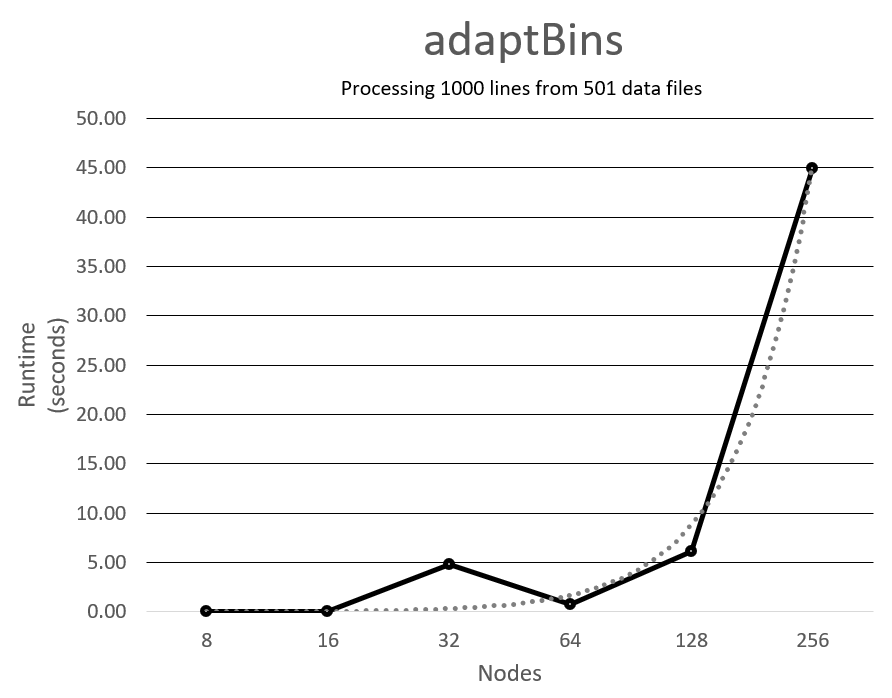
\includegraphics[width=0.8\textwidth]{adaptBins.png}

\subsection{swapData}

The \texttt{swapData} suffers from the same performance issues that \texttt{adaptBins} does. Both routines are heavily network dependent. Again, this routine needs to be tested on the cluster without any other workload to determine if the times reported are due to the algorithm's design or the network.

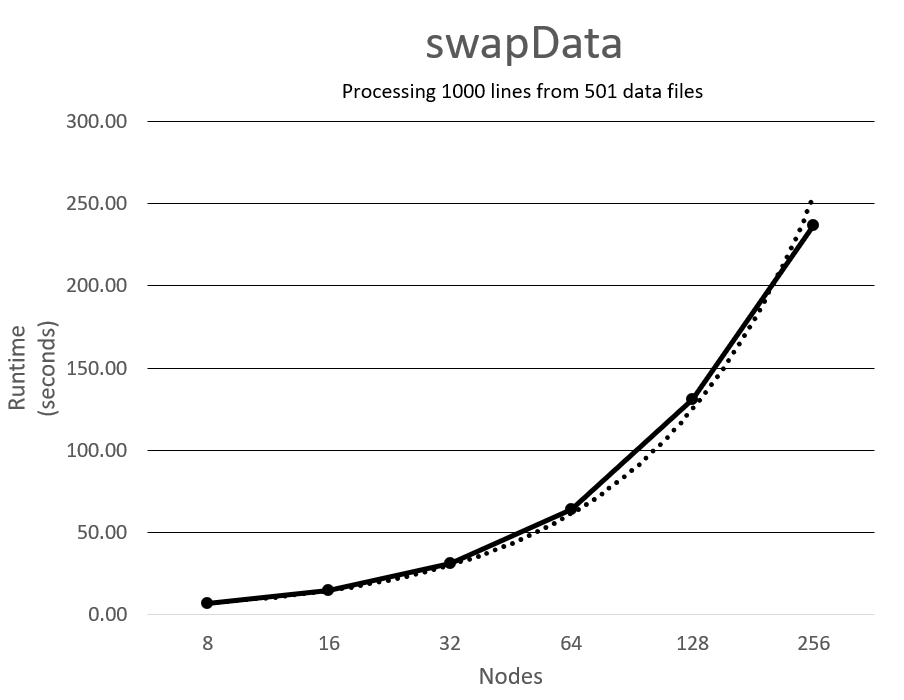
\includegraphics[width=0.8\textwidth]{swapData.png}


\subsection{Overall}

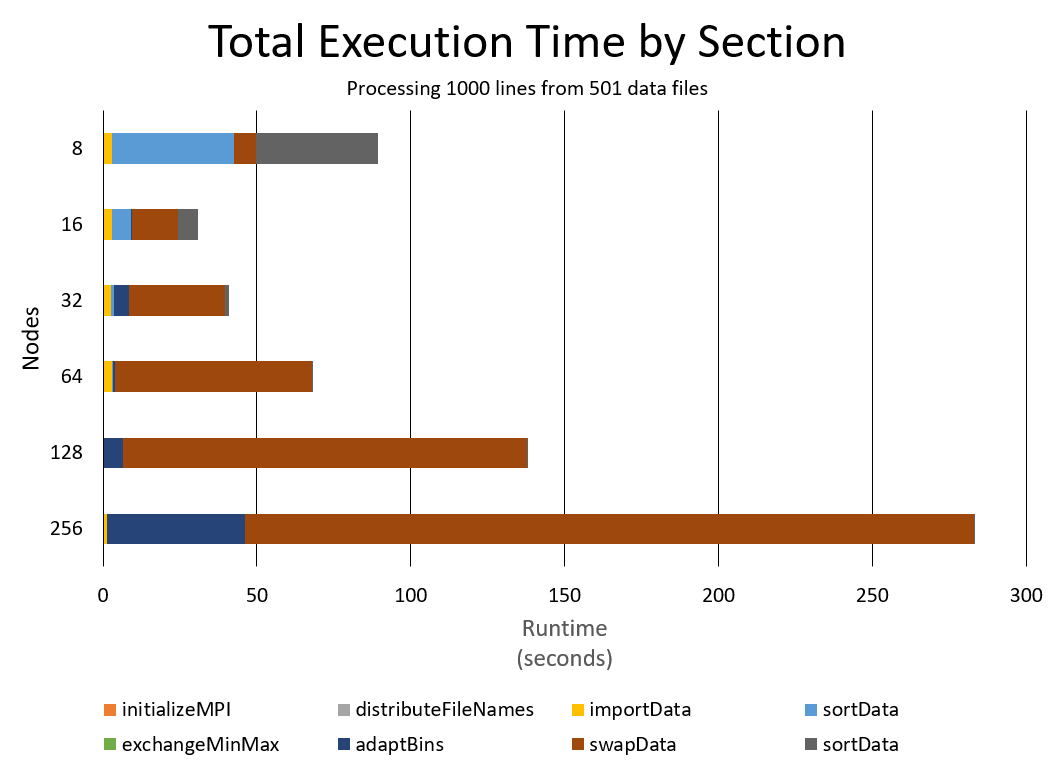
\includegraphics[width=0.8\textwidth]{totalTime.png}

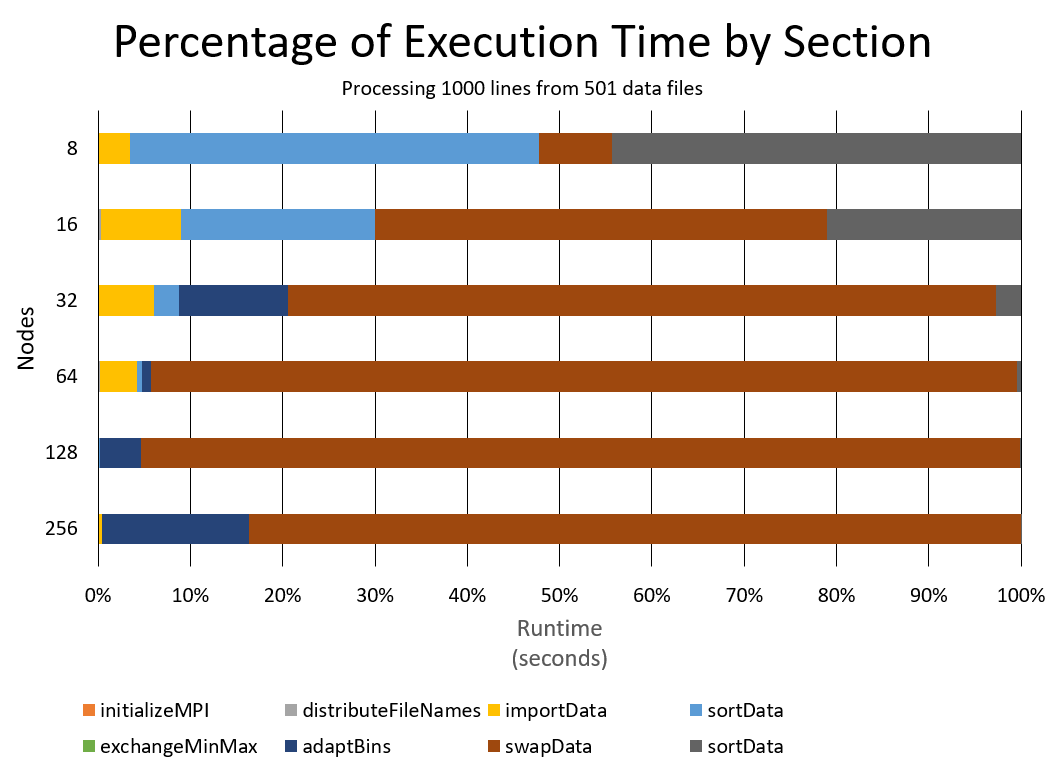
\includegraphics[width=0.8\textwidth]{percentTime.png}


\begin{tabular}{| c  r  r  r r|}
\hline
Nodes & initializeMPI & distributeFileNames & importData & sortData \\
\hline                                                          
256   & 0.00          & 0.25                & 0.95       & 0.03     \\
128   & 0.00          & 0.16                & 0.03       & 0.12     \\
64    & 0.00          & 0.13                & 2.74       & 0.35     \\
32    & 0.00          & 0.05                & 2.42       & 1.12     \\
16    & 0.00          & 0.10                & 2.66       & 6.46     \\
8     & 0.00          & 0.02                & 3.03       & 39.61    \\
 & & & & \\
\hline
Nodes &  exchangeMinMax & adaptBins & swapData & sortData  \\
\hline                                                     
256   &  0.00           & 44.96     & 236.75   & 0.03      \\
128   &  0.00           & 6.08      & 131.23   & 0.12      \\
64    &  0.00           & 0.72      &  63.98   & 0.35      \\
32    &  0.00           & 4.81      &  31.26   & 1.12      \\
16    &  0.00           & 0.02      &  15.05   & 6.46      \\
8     &  0.00           & 0.01      &   7.00   & 39.61     \\
 & & & & \\
\hline
Nodes & Total  & & & \\
\hline         
256   & 282.97 & & & \\
128   & 137.74 & & & \\
64    & 68.27  & & & \\
32    & 40.78  & & & \\
16    & 30.75  & & & \\
8     & 89.28  & & & \\
\hline
\end{tabular}
